%Mathematik 2
%Übungseinheit 3
%Hausübungen
%Aufgabe T1

\setcounter{T-section}{1}
\renewcommand*\thesection{T\Nummerierung{\arabic{T-section}}}
\section{Parallelprojektionen in die Aufrissebene}


a)\\
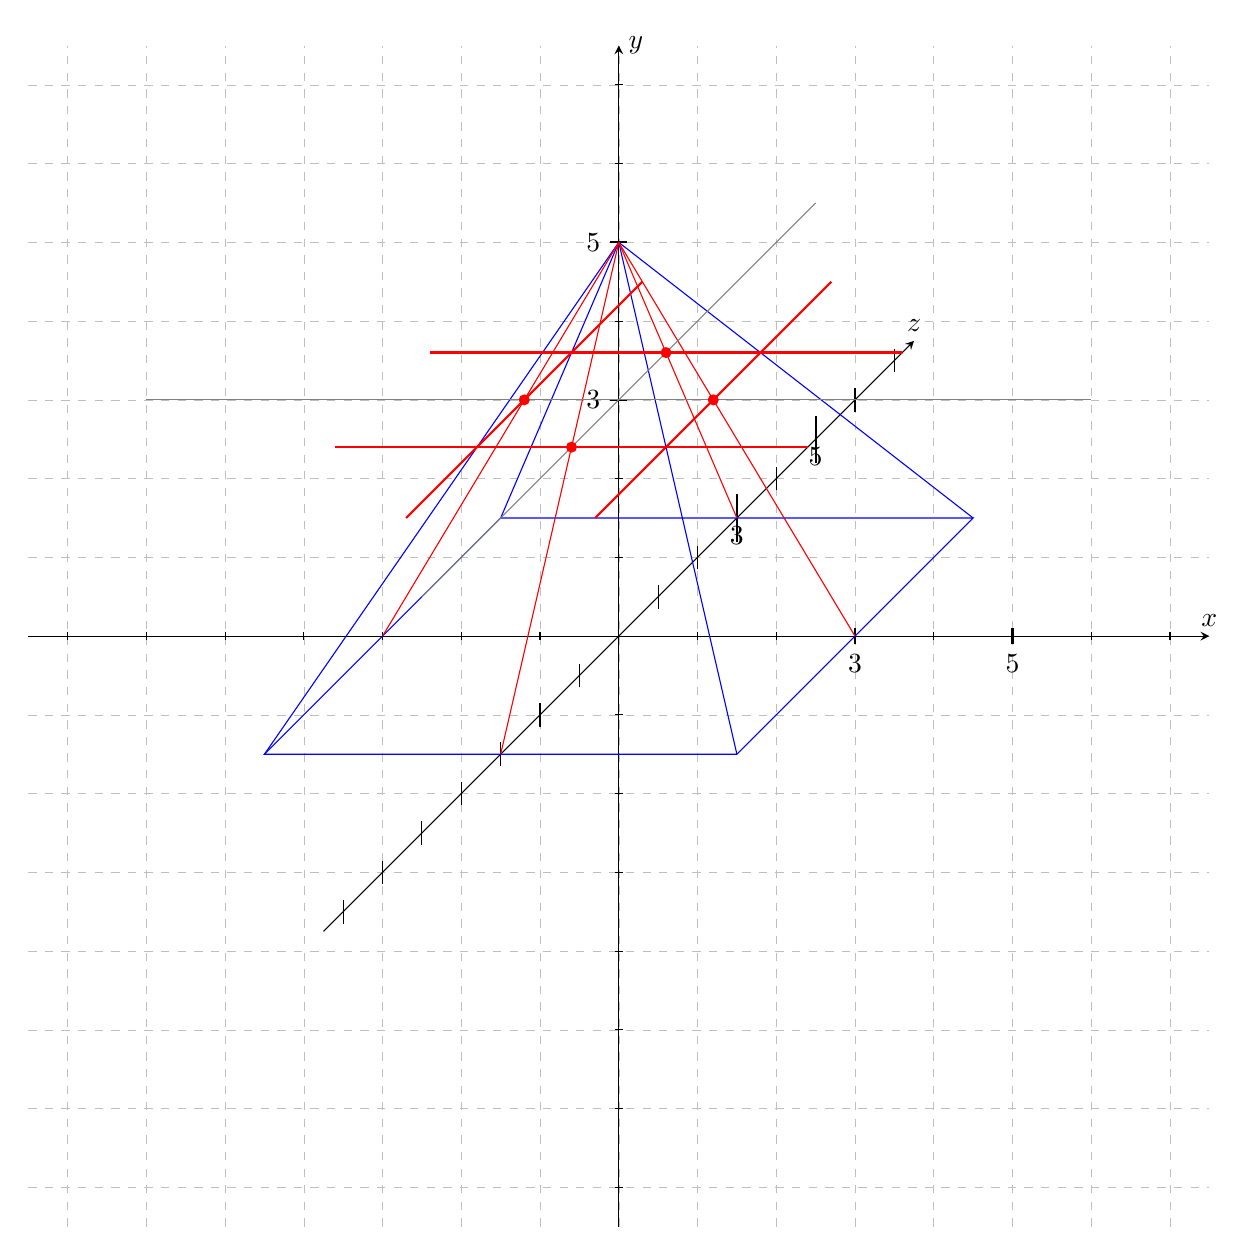
\begin{tikzpicture}[x=1cm,y=1cm,z=0.5cm,>=stealth]

\draw[step=1cm,lightgray,very thin,dashed] (-7.5,7.5) grid (7.5,-7.5);

% The axes
\draw[->] (xyz cs:x=-7.5) -- (xyz cs:x=7.5) node[above] {$x$};
\draw[->] (xyz cs:y=-7.5) -- (xyz cs:y=7.5) node[right] {$y$};
\draw[->] (xyz cs:z=-7.5) -- (xyz cs:z=7.5) node[above] {$z$};
% The thin ticks

\foreach \coo in {-7,...,7}
{
	\draw (\coo,-1.5pt) -- (\coo,1.5pt);
	\draw (-1.5pt,\coo) -- (1.5pt,\coo);
	\draw (xyz cs:y=-0.15pt,z=\coo) -- (xyz cs:y=0.15pt,z=\coo);
}

% The thick ticks
\foreach \coo in {3,5}
{
	\draw[thick] (\coo,-3pt) -- (\coo,3pt) node[below=6pt] {\coo};
	\draw[thick] (-3pt,\coo) -- (3pt,\coo) node[left=6pt] {\coo};
	\draw[thick] (xyz cs:y=-0.3pt,z=\coo) -- (xyz cs:y=0.3pt,z=\coo) node[below=8pt] {\coo};
}

\draw[blue] (xyz cs:x=-3,y=0,z=-3)--+(6,0,0)--+(6,0,6)--+(0,0,6)--cycle;
\draw[blue] (xyz cs:x=0,y=5,z=0)--+(-3,-5,-3);
\draw[blue] (xyz cs:x=0,y=5,z=0)--+(3,-5,3);
\draw[blue] (xyz cs:x=0,y=5,z=0)--+(3,-5,-3);
\draw[blue] (xyz cs:x=0,y=5,z=0)--+(-3,-5,3);


%Seitenhalbierende
\draw[red] (xyz cs:x=0,y=0,z=-3)coordinate(s_1)--(xyz cs:x=0,y=5,z=0)coordinate(s_11);
\draw[red] (xyz cs:x=3,y=0,z=0)coordinate(s_2)--+(-3,5,0)coordinate(s_22);
\draw[red] (xyz cs:x=0,y=0,z=3)coordinate(s_3)--+(0,5,-3)coordinate(s_33);
\draw[red] (xyz cs:x=-3,y=0,z=0)coordinate(s_4)--+(3,5,0)coordinate(s_44);

%verschieben des Koordinatensystems in Punkt 3
\draw[gray] (xyz cs:x=0,y=3,z=-5)coordinate(k_1)--(xyz cs:x=0,y=3,z=5)coordinate(k_11);
\draw[gray] (xyz cs:x=-6,y=3,z=0)coordinate(k_2)--(xyz cs:x=6,y=3,z=0)coordinate(k_22);

%Schnittpunkte Seitenhalbierende und Koordinatenachsen
\coordinate (c) at (intersection of s_1--s_11 and k_1--k_11);
\fill[red](c) circle(2pt);
\coordinate (d) at (intersection of s_2--s_22 and k_2--k_22);
\fill[red](d) circle(2pt);
\coordinate (e) at (intersection of s_3--s_33 and k_1--k_11);
\fill[red](e) circle(2pt);
\coordinate (f) at (intersection of s_4--s_44 and k_2--k_22);
\fill[red](f) circle(2pt);

\draw[red, thick] (c)--+(3,0,0)--+(-3,0,0);
\draw[red, thick] (e)--+(3,0,0)--+(-3,0,0);
\draw[red, thick] (d)--+(0,0,3)--+(0,0,-3);
\draw[red, thick] (f)--+(0,0,3)--+(0,0,-3);

\end{tikzpicture}\\
\usetikzlibrary{calc}
b)\\
\begin{tikzpicture}[x=1.5cm,y=1.5cm,z=0.75cm,>=stealth]

\draw[step=1.5cm,lightgray,very thin,dashed] (-5.5,5.5) grid (5.5,-5.5);

% The axes
\draw[->] (xyz cs:x=-5.5) -- (xyz cs:x=5.5) node[above] {$x$};
\draw[->] (xyz cs:y=-5.5) -- (xyz cs:y=5.5) node[right] {$z$};
\draw[->] (xyz cs:z=-5.5) -- (xyz cs:z=5.5) node[above] {$y$};
% The thin ticks

\foreach \coo in {-5,...,5}
{
	\draw (\coo,-5.5pt) -- (\coo,1.5pt);
	\draw (-5.5pt,\coo) -- (1.5pt,\coo);
	\draw (xyz cs:y=-0.15pt,z=\coo) -- (xyz cs:y=0.15pt,z=\coo);
}

% The thick ticks
\foreach \coo in {5}
{
	\draw[thick] (\coo,-3pt) -- (\coo,3pt) node[below=6pt] {\coo};
	\draw[thick] (-3pt,\coo) -- (3pt,\coo) node[left=6pt] {\coo};
	\draw[thick] (xyz cs:y=-0.3pt,z=\coo) -- (xyz cs:y=0.3pt,z=\coo) node[below=8pt] {\coo};
}

\draw[blue](xyz cs: x=0,y=-3,z=0)--+(3,0,0)--+(3,6,0)--+(-3,6,0)--+(-3,0,0)--cycle;
\draw[red] (0,0) circle (4.5cm);

\fill[red](xyz cs: x=3,y=0,z=0) circle(3pt);
\fill[red](xyz cs: x=-3,y=0,z=0) circle(3pt);

\fill[red](xyz cs: x=0,y=3,z=0) circle(3pt);
\fill[red](xyz cs: x=0,y=-3,z=0) circle(3pt);


\end{tikzpicture}\\
\pagebreak

c)\\

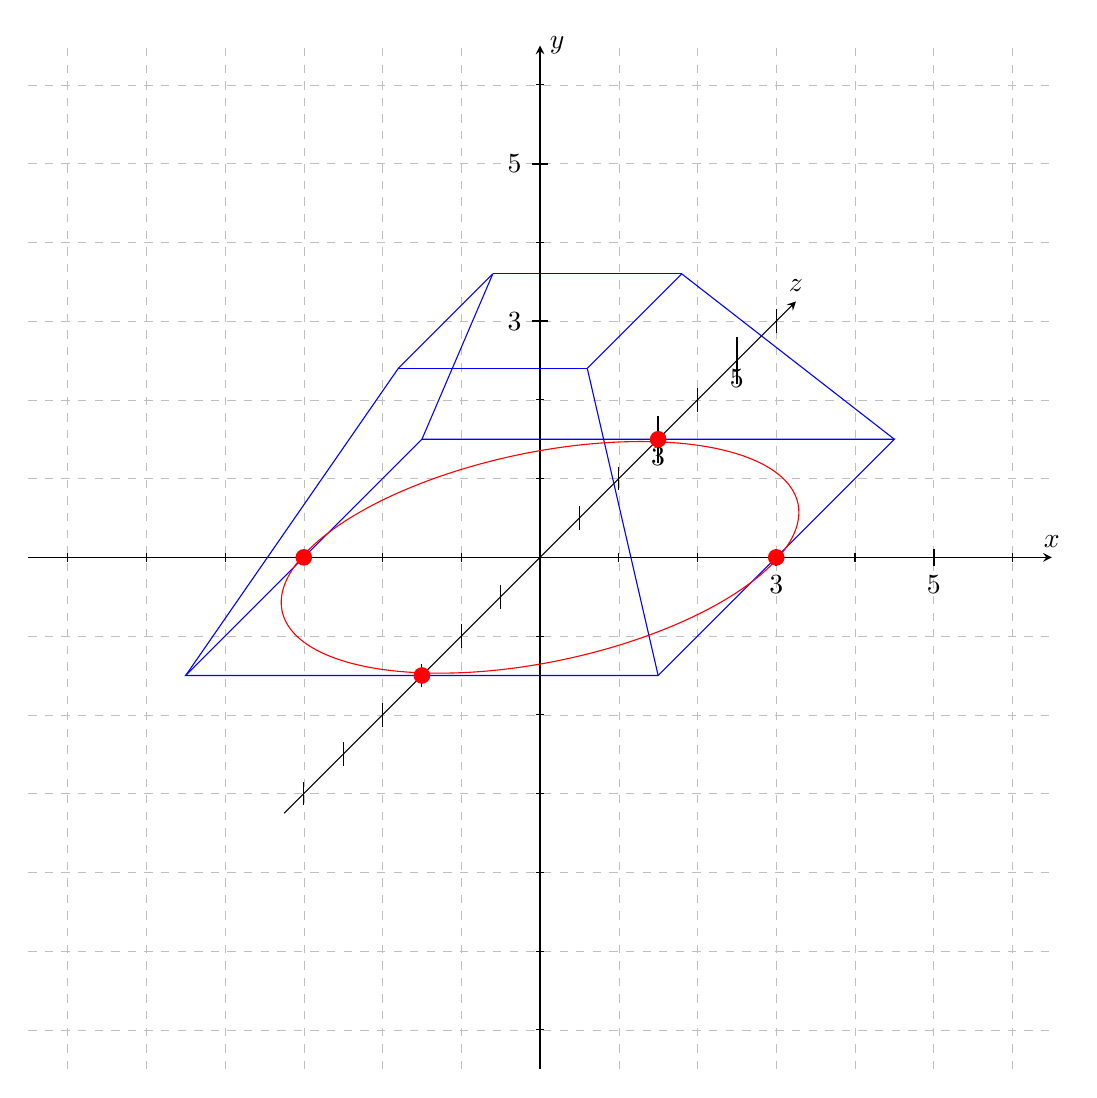
\begin{tikzpicture}[x=1cm,y=1cm,z=0.5cm,>=stealth]

\draw[step=1cm,lightgray,very thin,dashed] (-6.5,6.5) grid (6.5,-6.5);

% The axes
\draw[->] (xyz cs:x=-6.5) -- (xyz cs:x=6.5) node[above] {$x$};
\draw[->] (xyz cs:y=-6.5) -- (xyz cs:y=6.5) node[right] {$y$};
\draw[->] (xyz cs:z=-6.5) -- (xyz cs:z=6.5) node[above] {$z$};
% The thin ticks

\foreach \coo in {-6,...,6}
{
	\draw (\coo,-1.5pt) -- (\coo,1.5pt);
	\draw (-1.5pt,\coo) -- (1.5pt,\coo);
	\draw (xyz cs:y=-0.15pt,z=\coo) -- (xyz cs:y=0.15pt,z=\coo);
}

% The thick ticks
\foreach \coo in {3,5}
{
	\draw[thick] (\coo,-3pt) -- (\coo,3pt) node[below=6pt] {\coo};
	\draw[thick] (-3pt,\coo) -- (3pt,\coo) node[left=6pt] {\coo};
	\draw[thick] (xyz cs:y=-0.3pt,z=\coo) -- (xyz cs:y=0.3pt,z=\coo) node[below=8pt] {\coo};
}

\draw[blue] (xyz cs:x=-3,y=0,z=-3)--+(6,0,0)--+(6,0,6)--+(0,0,6)--cycle;

\draw[blue](xyz cs: x=-3,y=0,z=-3)--(xyz cs: x=-1.2,y=3,z=-1.2);
\draw[blue](xyz cs: x=3,y=0,z=-3)--(xyz cs: x=1.2,y=3,z=-1.2);
\draw[blue](xyz cs: x=3,y=0,z=3)--(xyz cs: x=1.2,y=3,z=1.2);
\draw[blue](xyz cs: x=-3,y=0,z=3)--(xyz cs: x=-1.2,y=3,z=1.2);

\draw[blue](xyz cs: x=-1.2,y=3,z=1.2)--(xyz cs: x=1.2,y=3,z=1.2);
\draw[blue](xyz cs: x=-1.2,y=3,z=-1.2)--(xyz cs: x=1.2,y=3,z=-1.2);
\draw[blue](xyz cs: x=-1.2,y=3,z=-1.2)--(xyz cs: x=-1.2,y=3,z=1.2);
\draw[blue](xyz cs: x=1.2,y=3,z=-1.2)--(xyz cs: x=1.2,y=3,z=1.2);

%\draw[red] (0,0,0) ellipse (3cm and 0cm and 1.5cm);
\begin{scope}[shift={(-1.2,-1.5))},x={(1.2,1.5)},y={($(-1.5,-1.5)!1!90:(1.5,1.5)$)}]
\draw[red] (1,0) ellipse (0.98 and 0.33);
\end{scope}

\fill[red](xyz cs: x=3,y=0,z=0) circle(3pt);
\fill[red](xyz cs: x=-3,y=0,z=0) circle(3pt);
\fill[red](xyz cs: x=0,y=0,z=-3) circle(3pt);
\fill[red](xyz cs: x=0,y=0,z=3) circle(3pt);


\end{tikzpicture}\\

\pagebreak

d)\\


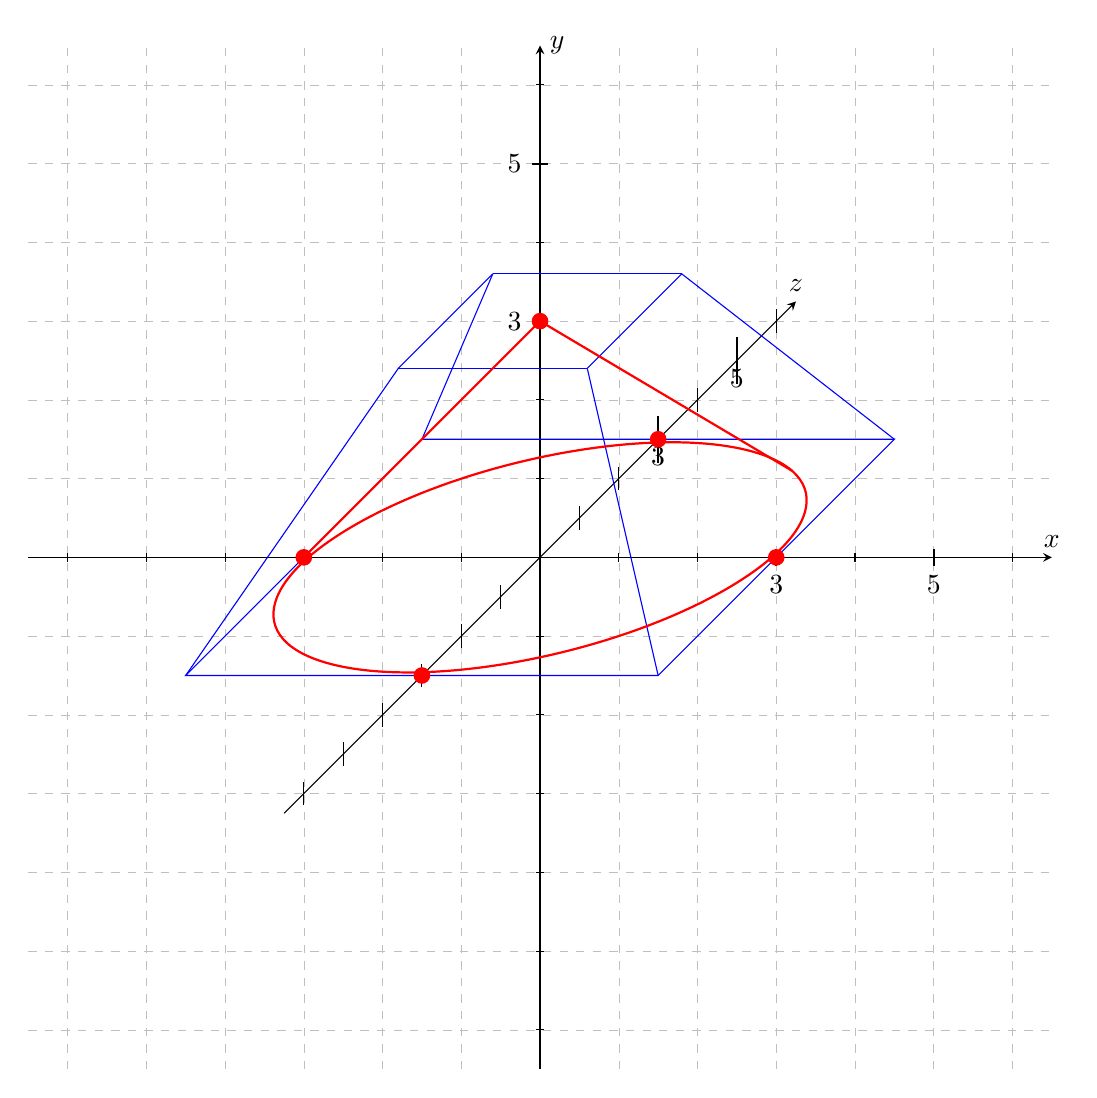
\begin{tikzpicture}[x=1cm,y=1cm,z=0.5cm,>=stealth]

\draw[step=1cm,lightgray,very thin,dashed] (-6.5,6.5) grid (6.5,-6.5);

% The axes
\draw[->] (xyz cs:x=-6.5) -- (xyz cs:x=6.5) node[above] {$x$};
\draw[->] (xyz cs:y=-6.5) -- (xyz cs:y=6.5) node[right] {$y$};
\draw[->] (xyz cs:z=-6.5) -- (xyz cs:z=6.5) node[above] {$z$};
% The thin ticks

\foreach \coo in {-6,...,6}
{
	\draw (\coo,-1.5pt) -- (\coo,1.5pt);
	\draw (-1.5pt,\coo) -- (1.5pt,\coo);
	\draw (xyz cs:y=-0.15pt,z=\coo) -- (xyz cs:y=0.15pt,z=\coo);
}

% The thick ticks
\foreach \coo in {3,5}
{
	\draw[thick] (\coo,-3pt) -- (\coo,3pt) node[below=6pt] {\coo};
	\draw[thick] (-3pt,\coo) -- (3pt,\coo) node[left=6pt] {\coo};
	\draw[thick] (xyz cs:y=-0.3pt,z=\coo) -- (xyz cs:y=0.3pt,z=\coo) node[below=8pt] {\coo};
}

\draw[blue] (xyz cs:x=-3,y=0,z=-3)--+(6,0,0)--+(6,0,6)--+(0,0,6)--cycle;

\draw[blue](xyz cs: x=-3,y=0,z=-3)--(xyz cs: x=-1.2,y=3,z=-1.2);
\draw[blue](xyz cs: x=3,y=0,z=-3)--(xyz cs: x=1.2,y=3,z=-1.2);
\draw[blue](xyz cs: x=3,y=0,z=3)--(xyz cs: x=1.2,y=3,z=1.2);
\draw[blue](xyz cs: x=-3,y=0,z=3)--(xyz cs: x=-1.2,y=3,z=1.2);

\draw[blue](xyz cs: x=-1.2,y=3,z=1.2)--(xyz cs: x=1.2,y=3,z=1.2);
\draw[blue](xyz cs: x=-1.2,y=3,z=-1.2)--(xyz cs: x=1.2,y=3,z=-1.2);
\draw[blue](xyz cs: x=-1.2,y=3,z=-1.2)--(xyz cs: x=-1.2,y=3,z=1.2);
\draw[blue](xyz cs: x=1.2,y=3,z=-1.2)--(xyz cs: x=1.2,y=3,z=1.2);


\begin{scope}[shift={(0,0))},x={(0.85,0.46)},y={($(-0.5,-0.3)!1!90:(0.5,0.3)$)}]
%\begin{scope}[shift={(-1.2,-1.5))},x={(1.2,1.5)},y={($(-1.5,-1.5)!1!90:(1.5,1.5)$)}]
%\draw[red,thick] (1,0) ellipse (0.98 and 0.33);
\draw[red,thick] (0,0) ellipse (3 and 1.5);
\end{scope}

%\draw[red,thick] (0,0) ellipse (3 and 1.5);

\fill[red](xyz cs: x=3,y=0,z=0) circle(3pt);
\fill[red](xyz cs: x=-3,y=0,z=0) circle(3pt);
\fill[red](xyz cs: x=0,y=0,z=-3) circle(3pt);
\fill[red](xyz cs: x=0,y=0,z=3) circle(3pt);

%Kegelstumpf
\fill[red](xyz cs: x=0,y=3,z=0) circle(3pt);
\draw[red,thick](xyz cs: x=0,y=3,z=0)--(xyz cs: x=-3,y=0,z=0);
\draw[red,thick](xyz cs: x=0,y=3,z=0)--(xyz cs: x=3.2,y=1.1,z=0);

\end{tikzpicture}\\


